\FloatBarrier
\chapter{Software Installation}
\label{sec::A_si}
Since all the software is freely available on GitHub, you can always find a build section within the provided readme file there. The links to the respective GitHub folders is provided within each following section. For the case of an error that may occur during the build procedure, do not hesitate to open an issue there. I will then help you to get the software running on your device.

\FloatBarrier
\section{Build the Pattern Generator}
\label{sec::A1_pg}
The pattern generator can be found on GitHub at the following \href{https://github.com/mhubii/nmpc_pattern_generator}{\underline{link}}. Proceed as described below.
\begin{enumerate}
	\item Make sure all dependencies are installed. The pattern generator only requires the necessary dependencies (section \ref{sec::A51_nd}). For communication with the real robot, one further needs the real robot and simulation dependencies (section \ref{sec::A52_rs}, and the simulation models \ref{sec::A4_sm}). For the deep learning support, it is further required to have the deep learning dependencies installed (section \ref{sec::A53_dl}).
	\item Clone the pattern generator from GitHub with
	\newline \inlinecode{}{https://github.com/mhubii/nmpc\_pattern\_generator.git}
	\item Then do one of the following steps
	\begin{enumerate}
		\item To just build the pattern generator, do
		\newline \inlinecode{}{mkdir build \&\& cd build}
		\newline \inlinecode{}{cmake ..}
		\newline \inlinecode{}{make}
		\item To build the pattern generator with communication to the real robot or the simulation do
		\newline \inlinecode{}{mkdir build \&\& cd build}
		\newline \inlinecode{}{cmake -DCMAKE\_BUILD\_WITH\_YARP=ON}
		\newline \inlinecode{}{make}
		\item To build the pattern generator with deep learning support do
		\newline \inlinecode{}{mkdir build \&\& cd build}
		\newline \inlinecode{}{cmake -DBUILD\_WITH\_LEARNING=ON \\} \newline  \inlinecode{}{-DCMAKE\_PREFIX\_PATH=/absolute/path/to/libtorch ..}
		\newline \inlinecode{}{make}
	\end{enumerate}
	\item This is not necessary, but you can then install or uninstall the pattern generator with
	\newline \inlinecode{}{make install}
	\newline \inlinecode{}{make uninstall}
\end{enumerate}
The pattern generator comes with some tests and examples. They can be executed as follows
\begin{enumerate}
	\item To run the tests do
	\newline \inlinecode{}{cd build/bin}
	\newline \inlinecode{}{./pattern\_generator\_tests}
	\item To run an example do
	\newline \inlinecode{}{cd build/bin}
	\newline \inlinecode{}{./nmpc\_pattern\_generator\_example}
	\item The results may be visualized with
	\newline \inlinecode{}{cd plot}
	\newline \inlinecode{}{python plot\_pattern.py}
\end{enumerate}

\FloatBarrier
\section{Build the Android Joystick App}
\label{sec::A2_aa}
The Joystick app can be found on GitHub at the following \href{https://github.com/mhubii/ijoy}{\underline{link}}. Proceed as described below.
\begin{enumerate}
	\item Clone the Android app from GitHub with
	\newline \inlinecode{}{git clone https://github.com/mhubii/ijoy.git}
	\item Copy the \inlinecode{}{.apk} file that you cloned from GitHub to your Android smartphone.
	\item Make sure your device allows installation of apps from unknown sources. Under Android 7:
	\begin{enumerate}
		\item Go to settings and open lock \inlinecode{}{screen\&security}.
		\item Find entry \inlinecode{}{unkown sources} and enable it.
	\end{enumerate}
	\item Find the \inlinecode{}{.apk} using the file browser of your choice and execute it (figure \ref{fig::A2_apk} (a) and (b)).
	\begin{figure}[h!]
		\centering
		\subcaptionbox{File browser.}%
		[.22\linewidth]{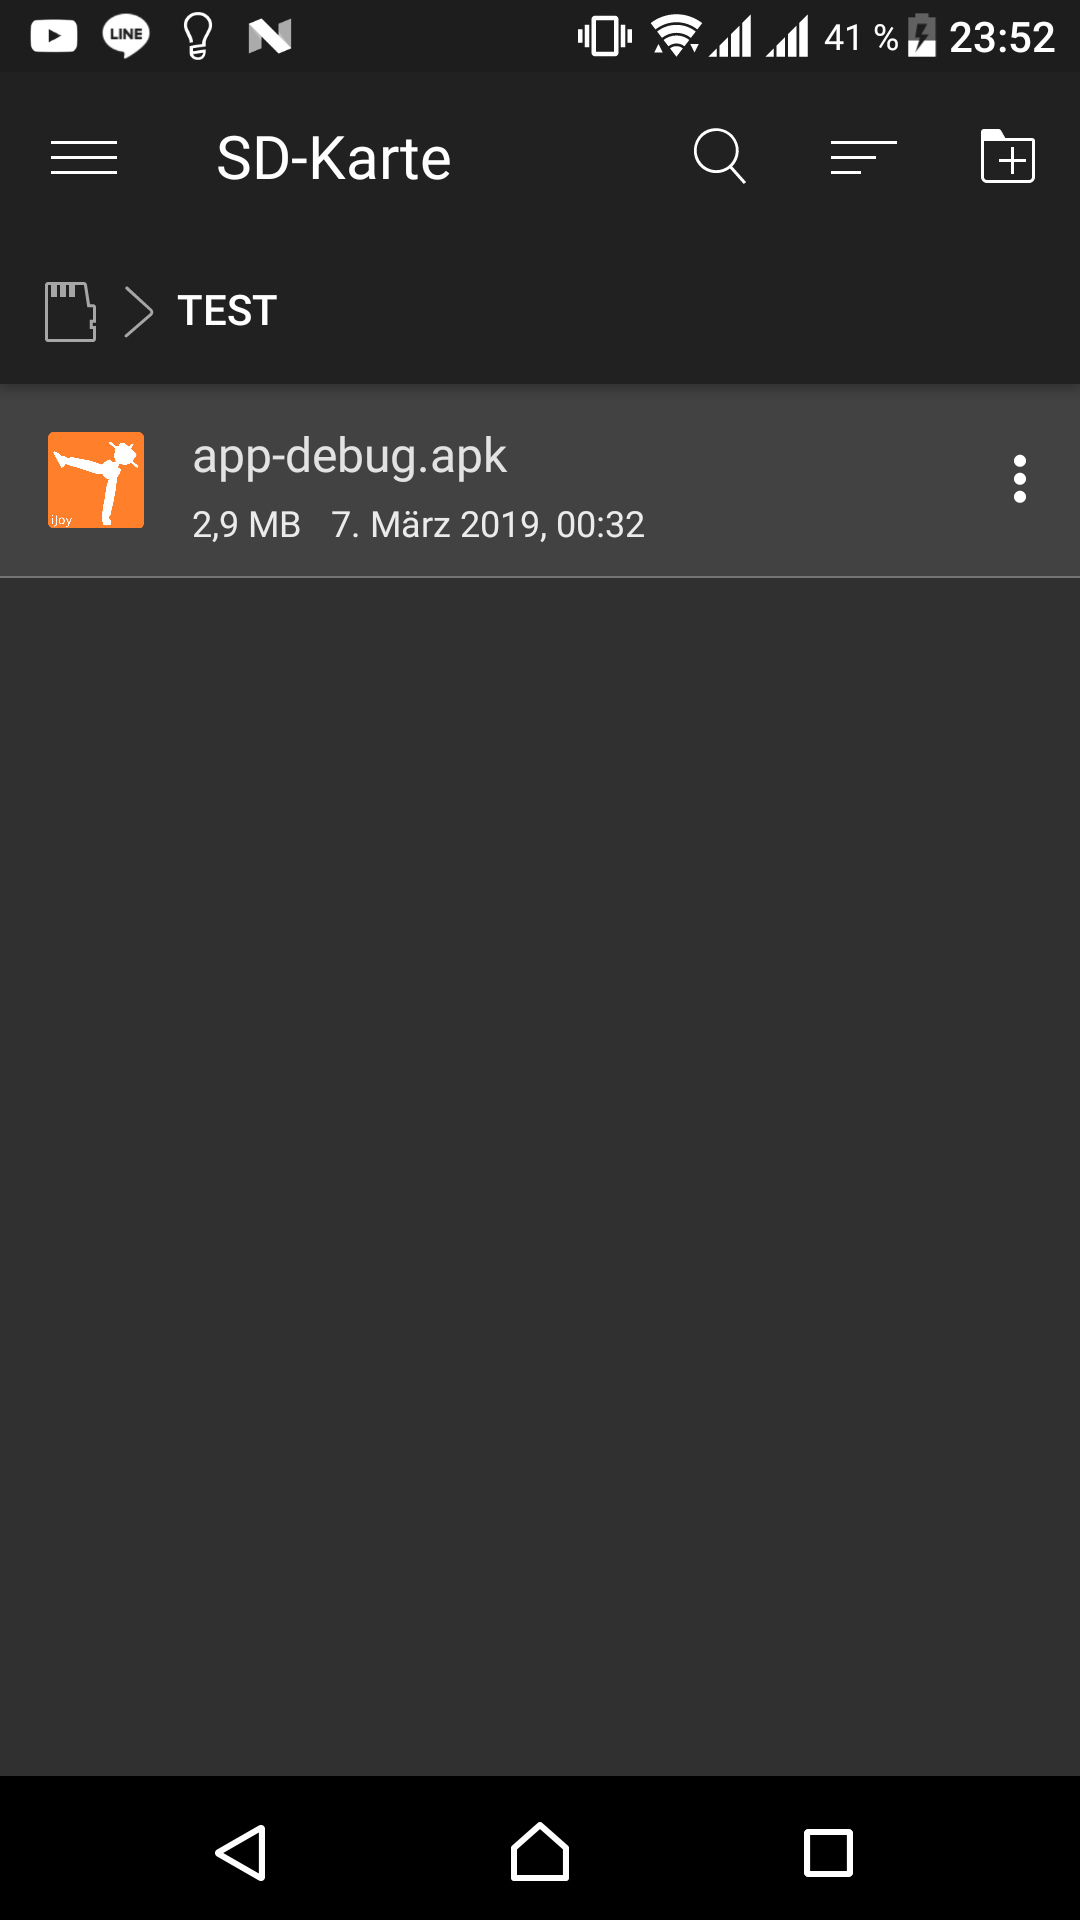
\includegraphics[scale=.06]{chapters/13_appendix/img/file_browser.png}}
		\subcaptionbox{Menu.}%
		[.22\linewidth]{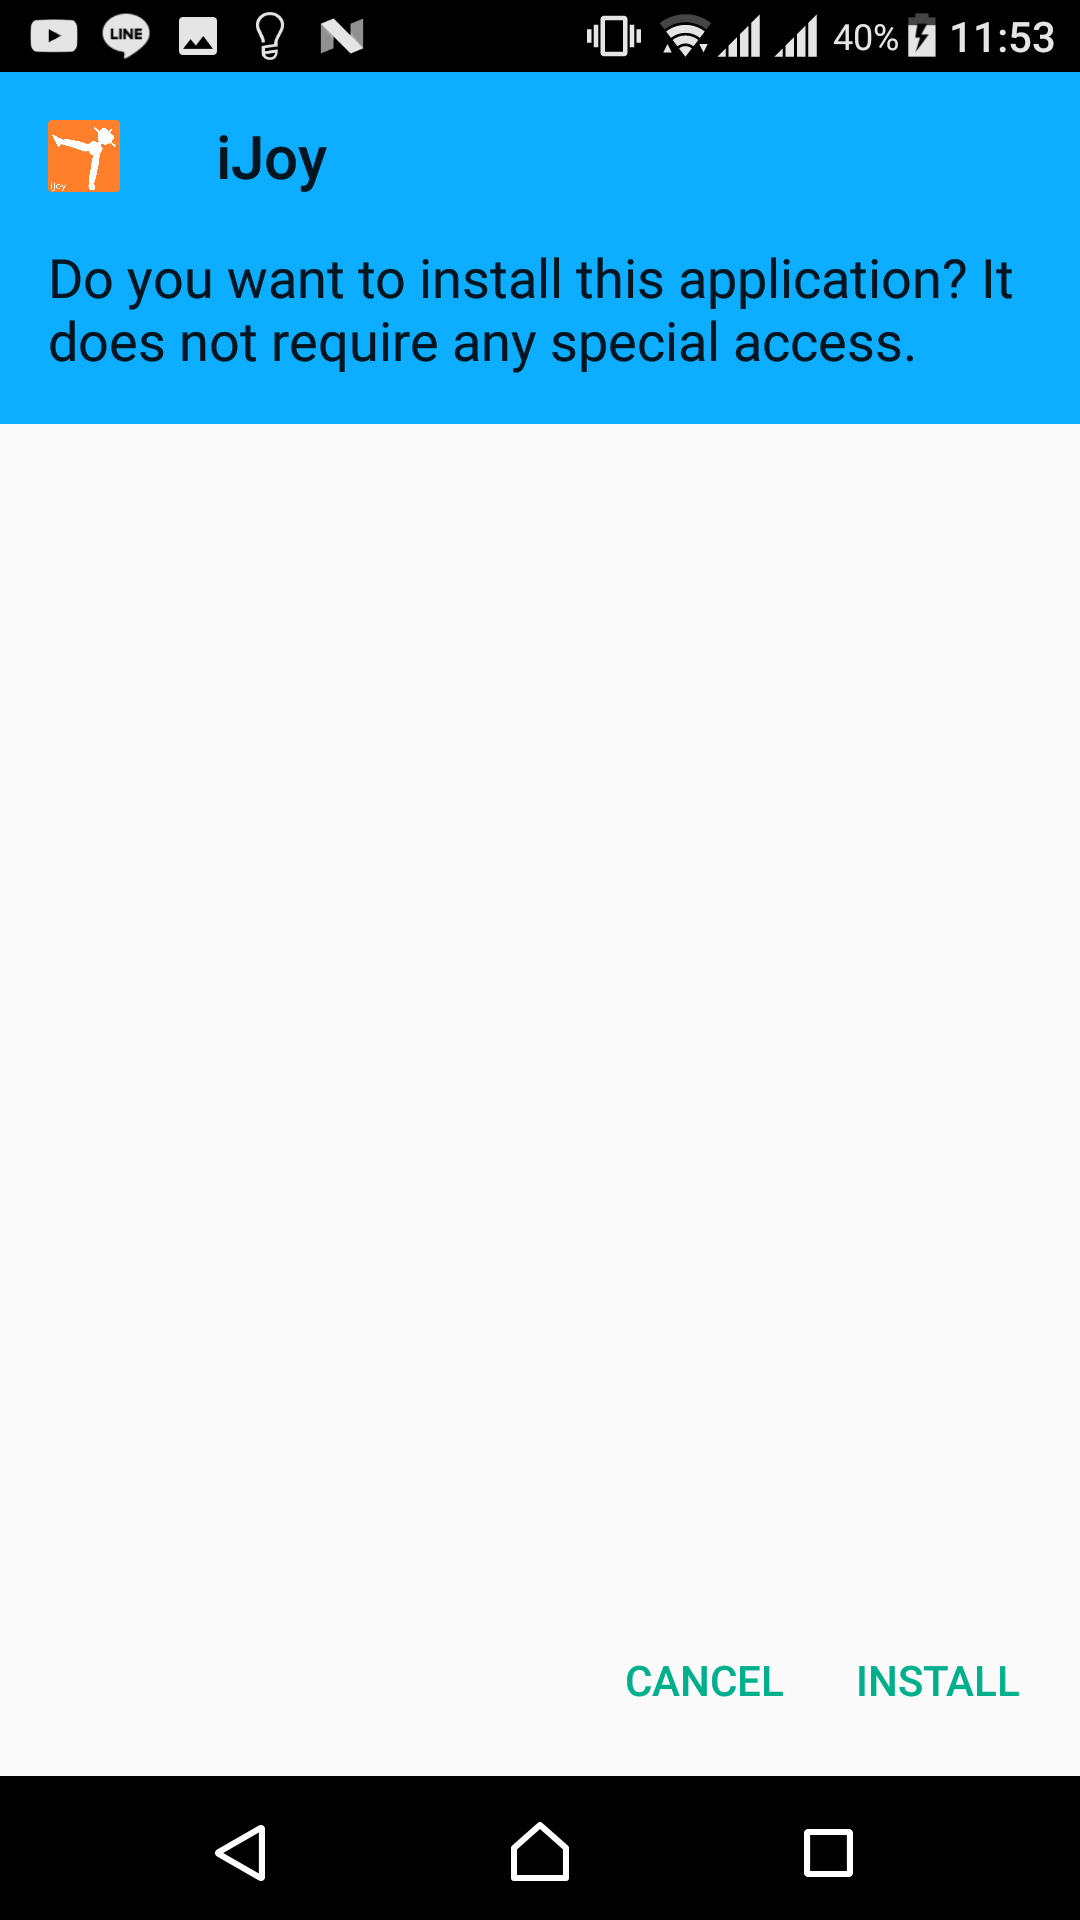
\includegraphics[scale=.06]{chapters/13_appendix/img/installation_start.png}}
		\subcaptionbox{Installing.}%
		[.22\linewidth]{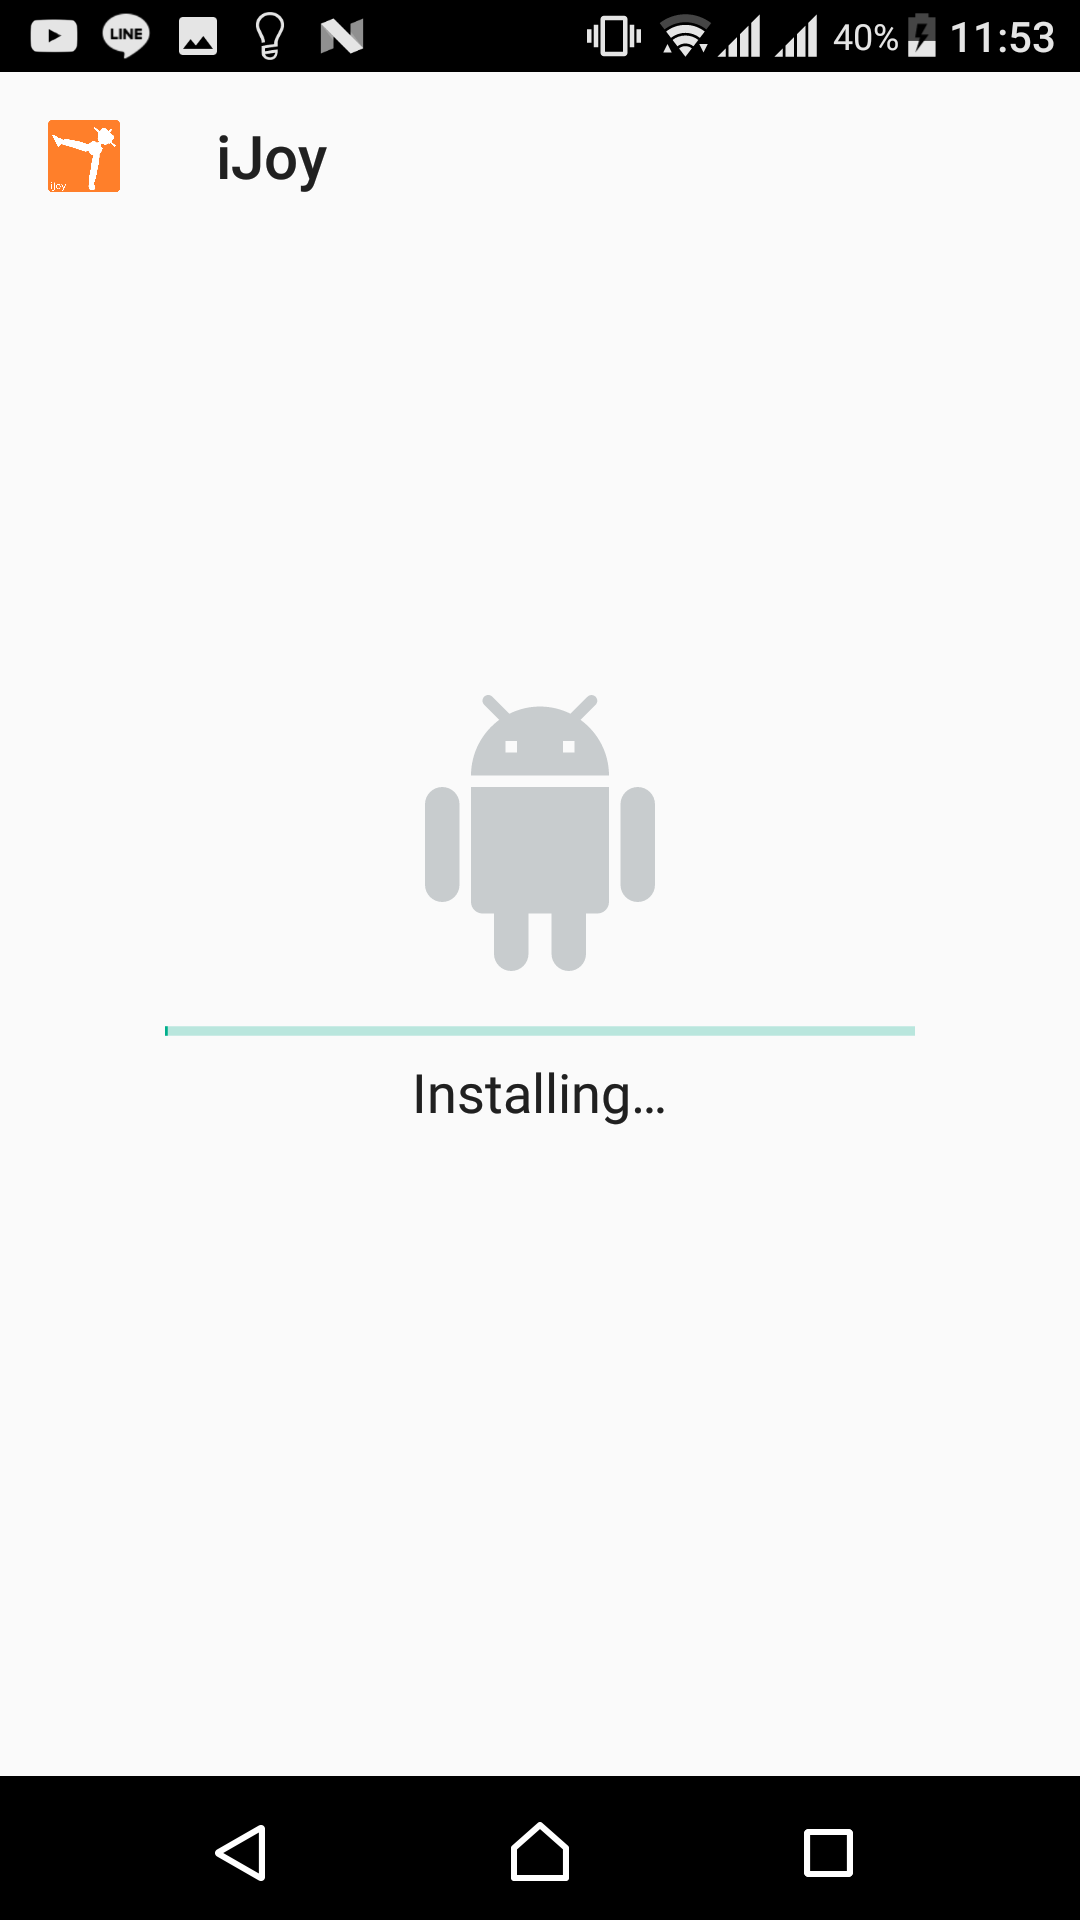
\includegraphics[scale=.06]{chapters/13_appendix/img/installation.png}}
		\subcaptionbox{Finished.}%
		[.22\linewidth]{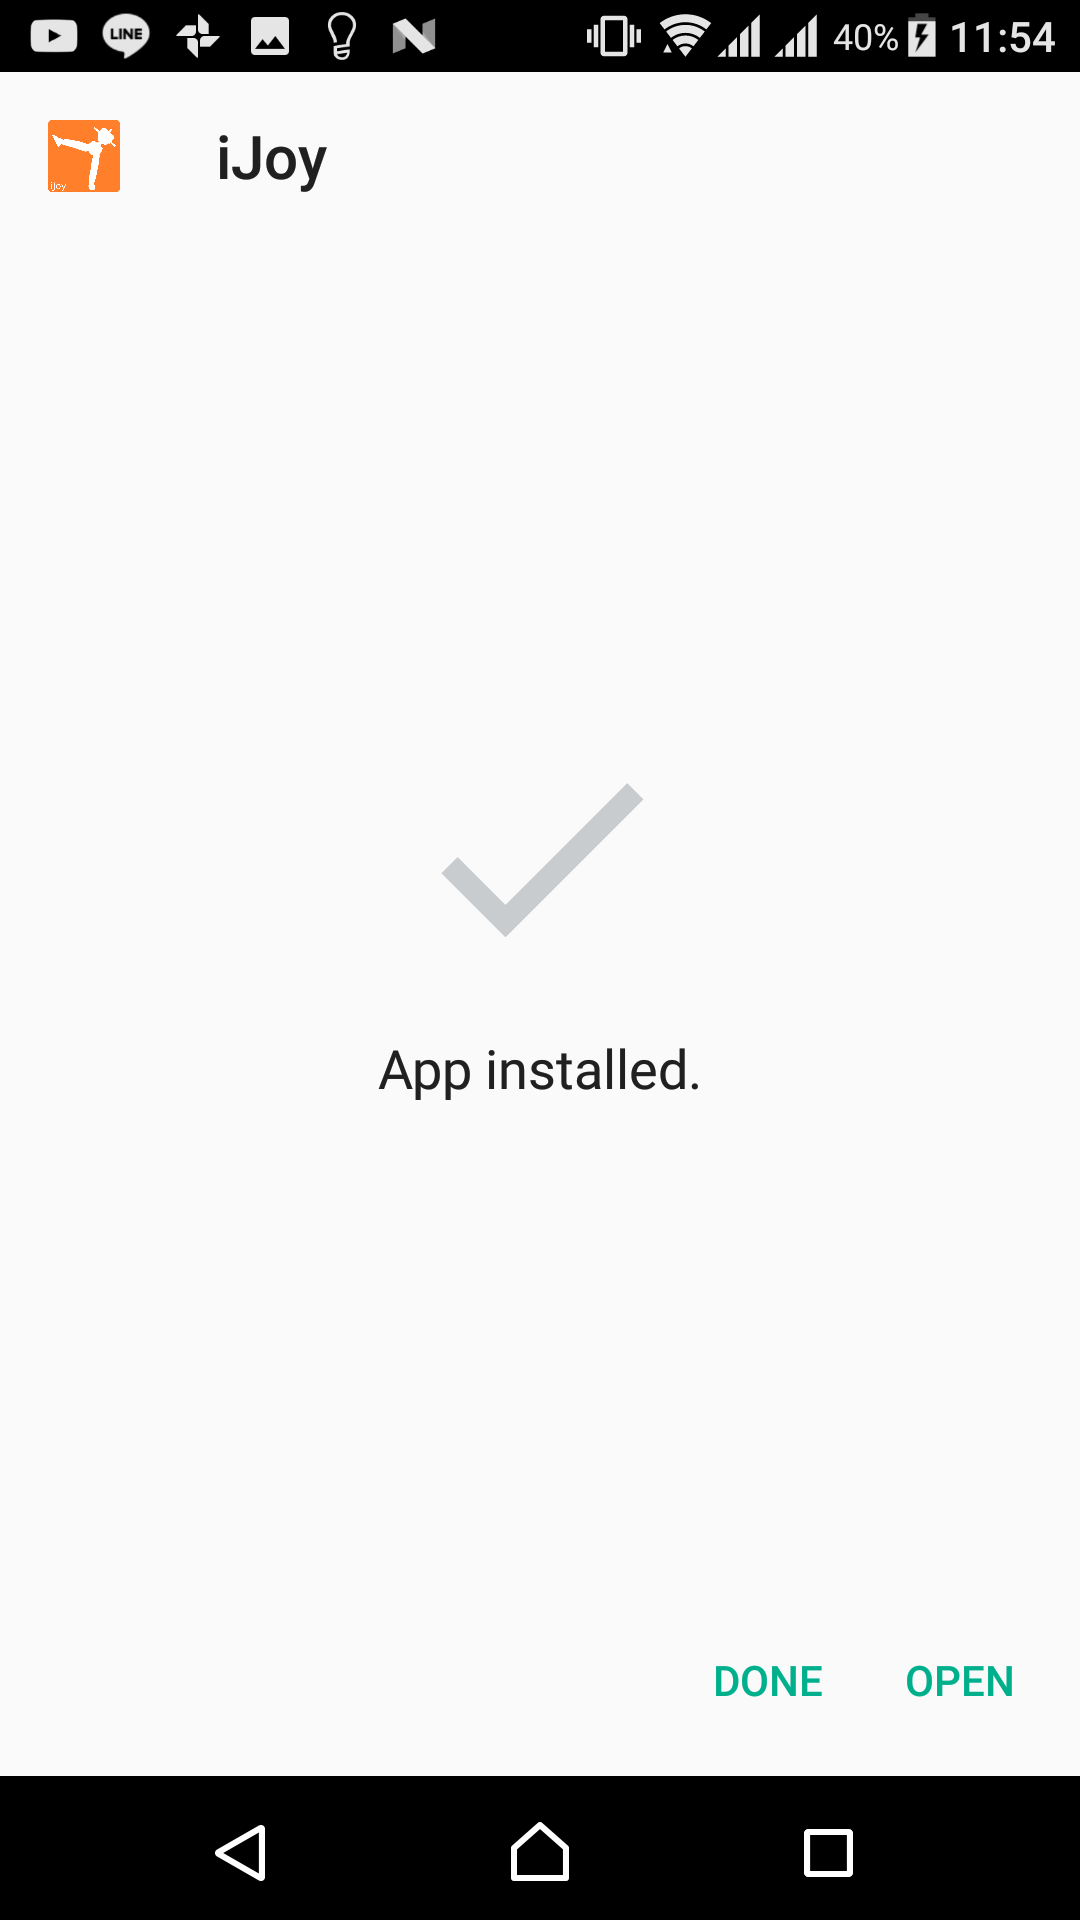
\includegraphics[scale=.06]{chapters/13_appendix/img/installation_end.png}}
		\caption{Installation process.}
		\label{fig::A2_apk}
	\end{figure}
	\item Follow the on-screen instructions and wait for the installation to finish (figure \ref{fig::A2_apk} (c) and (d)).
\end{enumerate}

\FloatBarrier
\section{Build Proximal Policy Optimization}
\label{sec::A3_pp}
The proximal policy optimization can be found on GitHub at the following \href{https://github.com/mhubii/ppo_libtorch}{\underline{link}}. Proceed as described below.
\begin{enumerate}
	\item Make sure the C++ API of PyTorch got install as described in section \ref{sec::A5_tp}.
	\item Clone proximal policy optimization from GitHub with
	\newline \inlinecode{}{git clone https://github.com/mhubii/ppo_libtorch.git}
	\item Then do
	\newline \inlinecode{}{mkdir build \&\& cd build}
	\newline \inlinecode{}{cmake -DCMAKE\_PREFIX\_PATH=/absolute/path/to/libtorch ..}
	\newline \inlinecode{}{make}
\end{enumerate}
You can then train and evaluate the neural network as described below.
\begin{enumerate}
	\item Train the neural network with
	\newline \inlinecode{}{cd build}
	\newline \inlinecode{}{./train\_ppo}
	\item Test the trained neural network with
	\newline \inlinecode{}{cd build}
	\newline \inlinecode{}{./test\_ppo}
	\item Visualize the results with
	\newline \inlinecode{}{python plot.py}
\end{enumerate}

\FloatBarrier
\section{Build Simulation Models}
\label{sec::A4_sm}
The simulation models can be found on GitHub at the following \href{https://github.com/mhubii/gazebo_models/}{\underline{link}}. Proceed as described below.
\begin{enumerate}
	\item Clone the models from GitHub with
	\newline \inlinecode{}{git clone https://github.com/mhubii/gazebo_models.git}
	\item You can either install the models to a location that Gazebo knows, or update the path, where Gazebo is looking for models.
	\item To update the path, add following line to your \inlinecode{}{bashrc}
	\newline \inlinecode{}{export GAZEBO\_MODEL\_PATH=<>/gazebo\_models:\$GAZEBO\_MODEL\_PATH}
	\newline Therein, replace \inlinecode{}{<>} by the location to which you cloned the repository.
	\item To install the models do
	\newline \inlinecode{}{mkdir build \&\& cd build}
	\newline \inlinecode{}{cmake -DCMAKE\_INSTALL\_PREFIX=~/.gazebo ..}
	\newline \inlinecode{}{make install}
	\item To uninstall the models do
	\newline \inlinecode{}{cd build}
	\newline \inlinecode{}{make uninstall}
\end{enumerate}

\FloatBarrier
\section{Build Third Party Software}
\label{sec::A5_tp}
The software that was developed as part of this thesis has some third-party dependencies, of which not all are necessary but required for some additional features.

\FloatBarrier
\subsection{Necessary Dependencies}
\label{sec::A51_nd}
These dependencies need to be installed.

\subsubsection{Eigen}
\begin{enumerate}
	\item The pattern generator is based on the blazingly fast Eigen library. To install it do
	\newline \inlinecode{}{sudo apt install libeigen3-dev}
	\item You may need to create a symbolic link
	\newline \inlinecode{}{sudo ln -s /usr/include/eigen3/Eigen/ /usr/include/}
	\newline \inlinecode{}{sudo ln -s /usr/include/eigen3/unsupported/ /usr/include/}
\end{enumerate}

\subsubsection{qpOASES}
To solve the sequential quadratic program, we need to install qpOASES. Please follow the \href{https://projects.coin-or.org/qpOASES/wiki/QpoasesInstallation}{\underline{install instructions}}, or head on as described below
\begin{enumerate}
	\item Download qpOASES
	\newline \inlinecode{}{wget https://www.coin-or.org/download/source/qpOASES/qpOASES-3.2.1.zip}
	\newline \inlinecode{}{unzip qpOASES-3.2.1.zip}
	\newline \inlinecode{}{cd qpOASES-3.2.1}
	\item Now since we want a shared library, in the \inlinecode{}{CMakeLists.txt} change 
	\newline \inlinecode{}{ADD\_LIBRARY(qpOASES STATIC \$\{SRC\})} to
	\newline \inlinecode{}{ADD\_LIBRARY(qpOASES SHARED \$\{SRC\})}
	\newline Then proceed with
	\newline \inlinecode{}{mkdir build \&\& cd build}
	\newline \inlinecode{}{cmake ..}
	\newline \inlinecode{}{make}
	\newline \inlinecode{}{sudo make install}
\end{enumerate}

\subsubsection{YAML}
The configurations are read in using the YAML file format. Run the command
\begin{enumerate}
	\item \inlinecode{}{sudo apt install libyaml-cpp-dev}
\end{enumerate}

\FloatBarrier
\subsection{Real Robot and Simulation Dependencies}
\label{sec::A52_rs}
To run the NMPC generator on a real robot or the simulation, we will need to install some more dependencies.

\subsubsection{Gazebo}
The simulation environment can be installed according to the \href{http://gazebosim.org/tutorials?tut=install_ubuntu&cat=install}{\underline{install instructions}}. The main steps are
\begin{enumerate}
	\item \inlinecode{}{sudo sh -c 'echo "deb http://packages.osrfoundation.org/gazebo/ubuntu-stable"\\}
	\newline \inlinecode{}{"`lsb\_release -cs` main" > /etc/apt/sources.list.d/gazebo-stable.list'}
	\newline \inlinecode{}{wget http://packages.osrfoundation.org/gazebo.key -O - | sudo apt-key add -}
	\newline \inlinecode{}{sudo apt-get update}
	\newline \inlinecode{}{sudo apt-get install gazebo9}
	\newline \inlinecode{}{sudo apt-get install libgazebo9-dev}
\end{enumerate}

\subsubsection{RBDL}
The rigid body kinematics are solved with RBDL. To install RBDL, do
\begin{enumerate}
	\item \inlinecode{}{hg clone https://bitbucket.org/rbdl/rbdl}
	\newline \inlinecode{}{cd rbdl}
	\newline \inlinecode{}{hg checkout dev}
	\newline \inlinecode{}{mkdir build \&\& cd build}
	\newline \inlinecode{}{cmake -DCMAKE\_BUILD\_TYPE=Release \\}
	\newline \inlinecode{}{-DRBDL\_BUILD\_ADDON\_URDFREADER=ON ..}
\end{enumerate}

\subsubsection{YARP}
\label{sec::a52_yarp}
Additionally, for communicating with the real robot, or the simulation, we need YARP. To install YARP, follow the \href{https://www.yarp.it/install.html}\underline{{installation instructions}}, or head on as described below
\begin{enumerate}
	\item \inlinecode{}{git clone https://github.com/robotology/yarp.git}
	\newline \inlinecode{}{cd yarp \&\& mkdir build \&\& cd build}
	\item If you have previously installed Anaconda, YARP may complain here. Go and install OpenCV within your Anaconda distribution
	\newline \inlinecode{}{# activate your anaconda environment, if you followed the}
	\newline \inlinecode{}{# instructions before in PyTorch, do conda activate py37\_torch}
	\newline \inlinecode{}{conda install opencv}
	\item Then do
	\newline \inlinecode{}{cmake -DOpenCV\_DIR=\$HOME/anaconda3/envs/py37\_torch/share/OpenCV ..}
	\newline \inlinecode{}{make}
	\newline \inlinecode{}{sudo make install}
\end{enumerate}

\subsubsection{Gazebo YARP Plugins}
\label{sec::a52_plugins}
Plugins for Gazebo are used to clone the behavior of the real robot into the simulation environment. Proceed as below
\begin{enumerate}
	\item \inlinecode{}{git clone https://github.com/robotology/gazebo-yarp-plugins.git}
	\newline \inlinecode{}{cd gazebo-yarp-plugins}
	\newline \inlinecode{}{mkdir build \&\& cd build}
	\newline \inlinecode{}{cmake -DCMAKE\_INSTALL\_PREFIX=\$HOME/gazebo-yarp-plugins ..}
	\newline \inlinecode{}{make}
	\newline \inlinecode{}{make install}
	\item Next, you need to tell Gazebo where to find the plugins, therefore add following to the \inlinecode{}{bashrc}
	\newline \inlinecode{}{export GAZEBO\_PLUGIN\_PATH=\$\{GAZEBO\_PLUGIN\_PATH\}}
	\newline \inlinecode{}{:\$HOME/gazebo-yarp-plugins/lib}
\end{enumerate}

\subsubsection{Gazebo Models}
The models are used within the simulation environment Gazebo. See section \ref{sec::A4_sm}.

\subsubsection{NCurses}
For the visualization of the control panel, we need to install ncurses, do
\begin{enumerate}
	\item \inlinecode{}{sudo apt install libncurses5-dev}
\end{enumerate}

\FloatBarrier
\subsection{Deep Learning Dependencies}
\label{sec::A53_dl}
To learn Nonlinear Model Predictive Control or simple navigation on top of Nonlinear Model Predictive Control, we will need to install PyTorch. For PyTorch to work in combination with RBDL, we need a source installation. Please check out this \href{https://gist.github.com/mhubii/1c1049fb5043b8be262259efac4b89d5}{\underline{gist}} to figure out how to perform a clean setup.
